\section{Extant experimental data}
\label{sec:database}

	We have data from the following two extant studies, which differ by their loading conditions and specimen orientation. 
	In the study by Sun \textit{et al}.\cite{sun_response_2004}, exogenously crosslinked BP patches were loaded along the preferred collagen fiber direction (PD) at a peak strain of 16\% and held constant for up to 65 million cycles (Fig. \ref{fig:database}A\&B). 
	The reference configurations of the exogenously crosslinked BP were tracked using fiducial markers attached to the center of the specimens\cite{sacks_biaxial_2000}. 
	The mechanical cycling was stopped at 30 and 65 million cycles for mechanical testing with multiple protocols and different loading paths. 
	It was found that there were significant extensions in the direction of loading (7.1\%), PD, and contractions in the cross direction (-7.7\%). 
	In addition, the collagen fiber crimp period increase from 40.6$\mu$m to 45.24$\mu$m which is consistent with the convection of the collagen fiber architecture that would occur as collagen fiber straighten (Fig. \ref{fig:PS}D). 
	The mechanical response also changes accordingly. 
	The compliance in the PD decreased over time while the compliance in the cross direction of the tissue increased. 

	In the study by Sellaro \textit{et al}.\cite{sellaro_effects_2007}, the same exogenously crosslinked BP patches were cycled at 500kPa for up to 50 million cycles (Fig. \ref{fig:database}C\&D). 
	In this case, the specimens were separated into two groups: with stress controlled loading along the 1) PD and 2) orthogonal to the PD (XD). 
	Similarly, the reference states of the exogenously crosslinked BP specimens were tracked, with cycling stopped at 20 and 50 million cycles for mechanical testing. 
	Analysis of the results shown interesting differences between the PD and XD cycled specimens. 
	For both the PD and XD cycled specimens, we observed significant elongation in the direction of loading and contraction in the orthogonal direction with cycling. 
	Additionally, the effective stiffness in the direction of loading increased over time, whereas the orthogonal direction decreased over time. 
	For the PD cycled specimens, it was observed that the collagen fiber orientation distribution became more aligned, and the collagen fiber crimp period increased from 24 $\mu$m to 28$\mu$m. 
	On the other hand, for the XD cycled specimens, it was observed that the collagen fiber orientation distribution became more spread, and the collagen fiber crimp period remained unchanged. 
	These structural changes with direction of cycling are consistent with the structural convection that would occur according to the dimensional changes (Fig. \ref{fig:PS}C\&D). 

\begin{figure}[hbt]
\centering
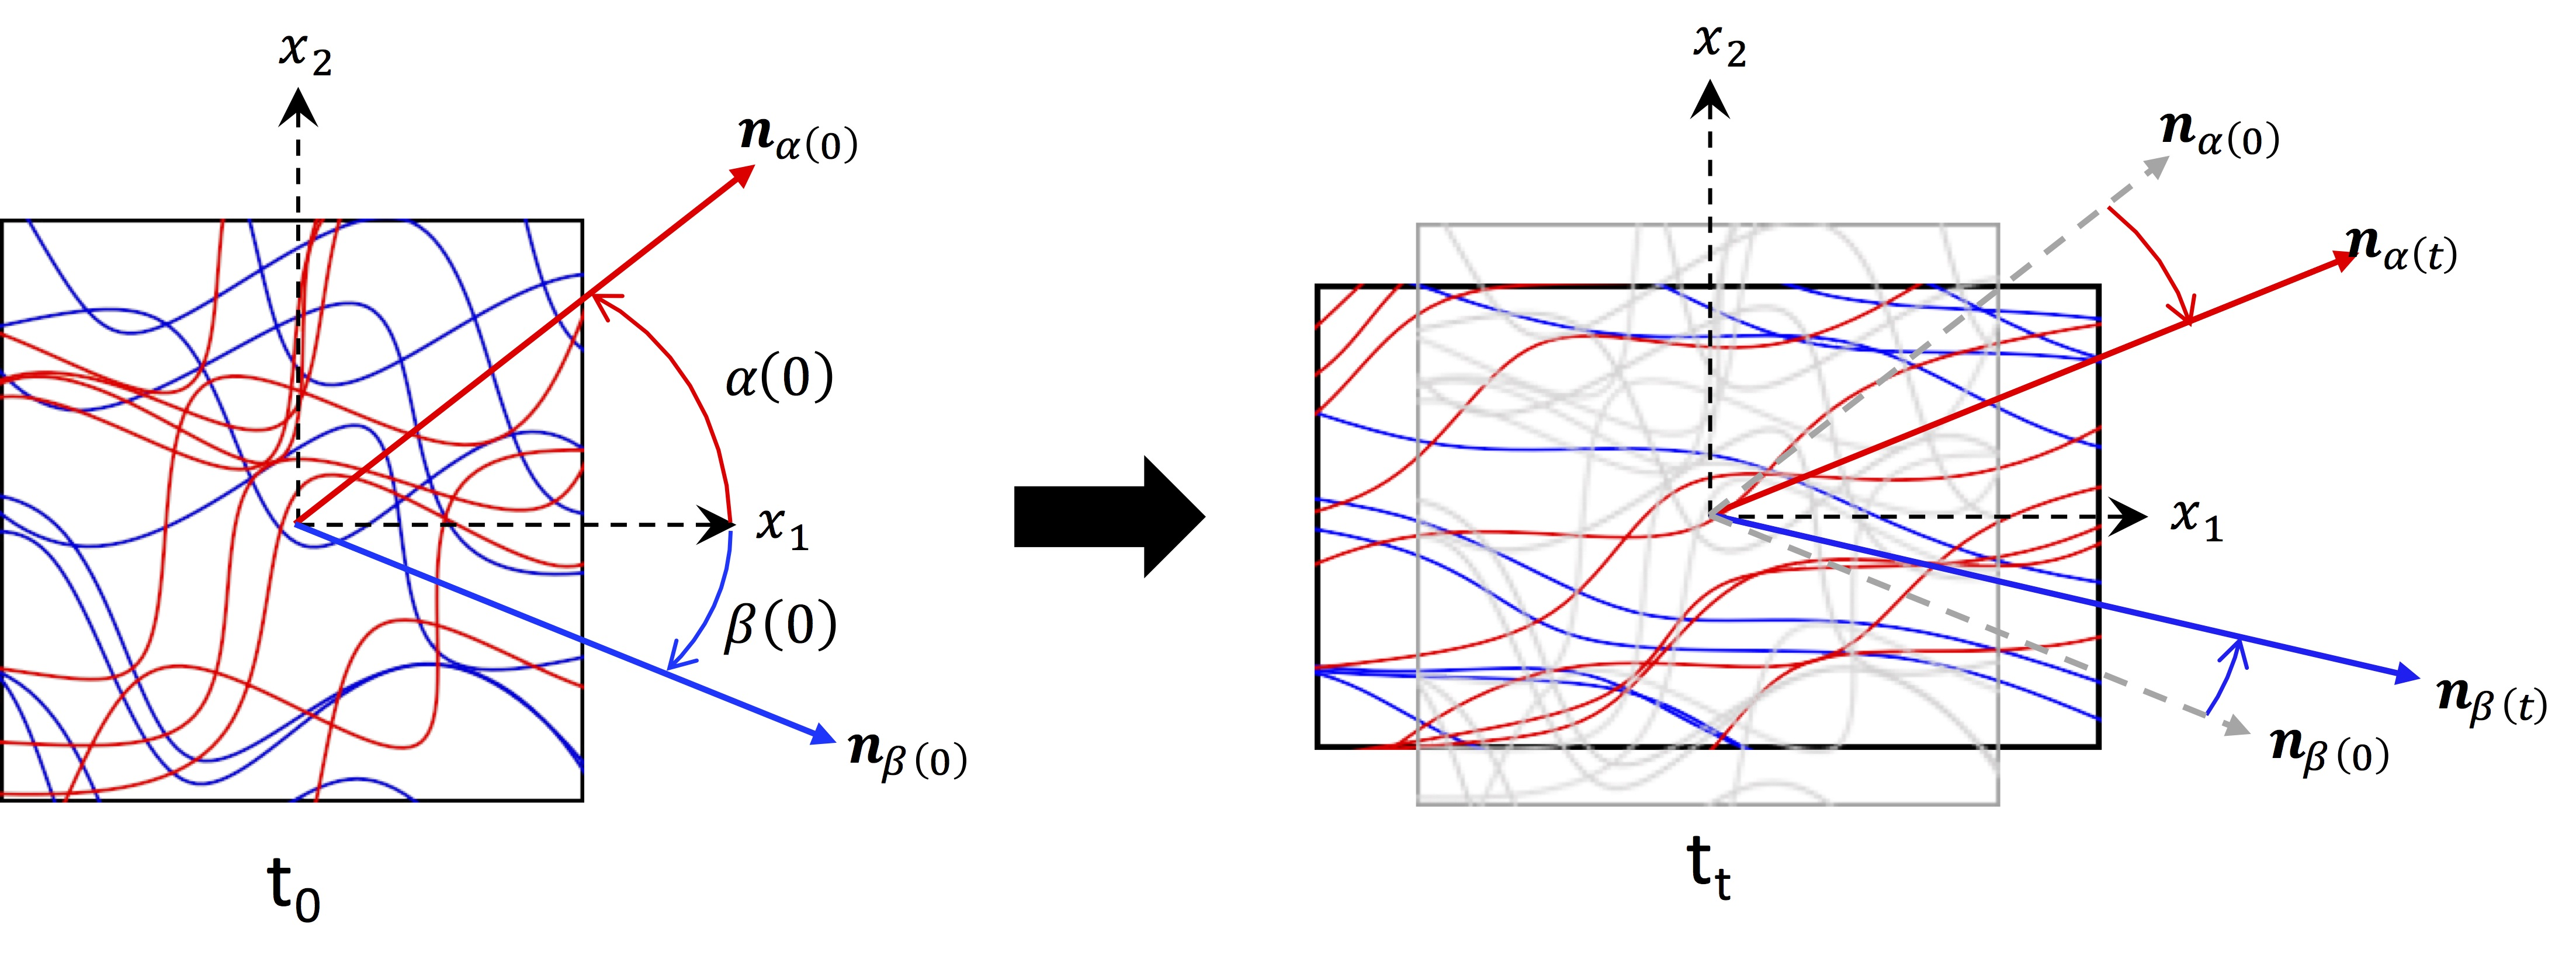
\includegraphics[width=0.6\paperwidth]{Images/chapter4/figure4}
\caption{We utilize two extant databases in this study. The first is strain controlled, with A) constant strain level and is B) sorted for orientation along the preferred direction then put through cyclic loading and mechanical testing. The second is with C) constant strain but evolving strain level. The specimens are then D) sorted for orientation along both the preferred direction and cross-preferred direction, then put through cyclic loading and mechanical testing.}
\label{fig:database}
\end{figure}